\documentclass[a4paper]{article}
\usepackage[warn]{mathtext}
\usepackage[utf8]{inputenc}
\usepackage[T2A]{fontenc}
\usepackage[english,russian]{babel}
\usepackage{booktabs}
\usepackage{multicol}
\usepackage{fancyhdr}
\usepackage{graphicx}
\usepackage{microtype}
\usepackage{wrapfig}
\usepackage{amsmath}
\usepackage{floatflt}
\usepackage{geometry} \geometry{verbose,a4paper,tmargin=2cm,bmargin=2cm,lmargin=1.5cm,rmargin=1.5cm}
\usepackage{float}
\usepackage{amssymb}
\usepackage{caption}
\usepackage{epsfig}
\usepackage{newunicodechar}
\usepackage{color}

\begin{document}

\graphicspath{ {pictures/} }
\begin{center}
    {\scshape\Large Лабораторная работа по квантовой электронике} \par

    \

    {\huge\bfseries № 23 Инжекционные полупроводниковые лазеры} \par 

    \

    {\large Яромир Водзяновский Б04-855а}
\end{center}

\

\
\section{Описание работы}

    \subsection{Цели}
        
        \par В ходе работы предлагается решить следующие поставленные задачи:
        
        \begin{enumerate}
            \item Измерение спектральных характеристик лазера и светодиодов, их дальнейший анализ
            \item Получение зависимости мощности излучения светодиодов и лазера от мощности накачки (Вт-Вт характеристика)
        \end{enumerate}
        
    \subsection{Суть эксперимента}
        \subsubsection{Спектральная характеристика}
            
            \par Исследование зависимости спеткра излучения инжекционного полупроводникового лазера/светодиодов от мощности накачки производится путём изменения детектируемой длины волны и фиксации напряжения при постоянной мощност накачки.
            \par Для лазера опыт производится четыре раза при разных накачках с целью определения характера изменения формы спектральной характеристики от установленной мощности накачки.
            
        \subsubsection{Ватт-Ваттная характеристика}
        
            \par Получение зависимости мощности излучения от мощности накачки для светодиодов и лазера реализуется поточечным изменением тока и напряжения накачки и фиксации установившихся тока и напряжения
    
\section{Экспериментальные данные}
    \subsection{Спектральные характеристики}
    
        \par \textit{Рассмотрим зависимость аплитуды излучения лазера от длины волны при разных токах накачки}
        
        \begin{figure}[H]
            \begin{center}
                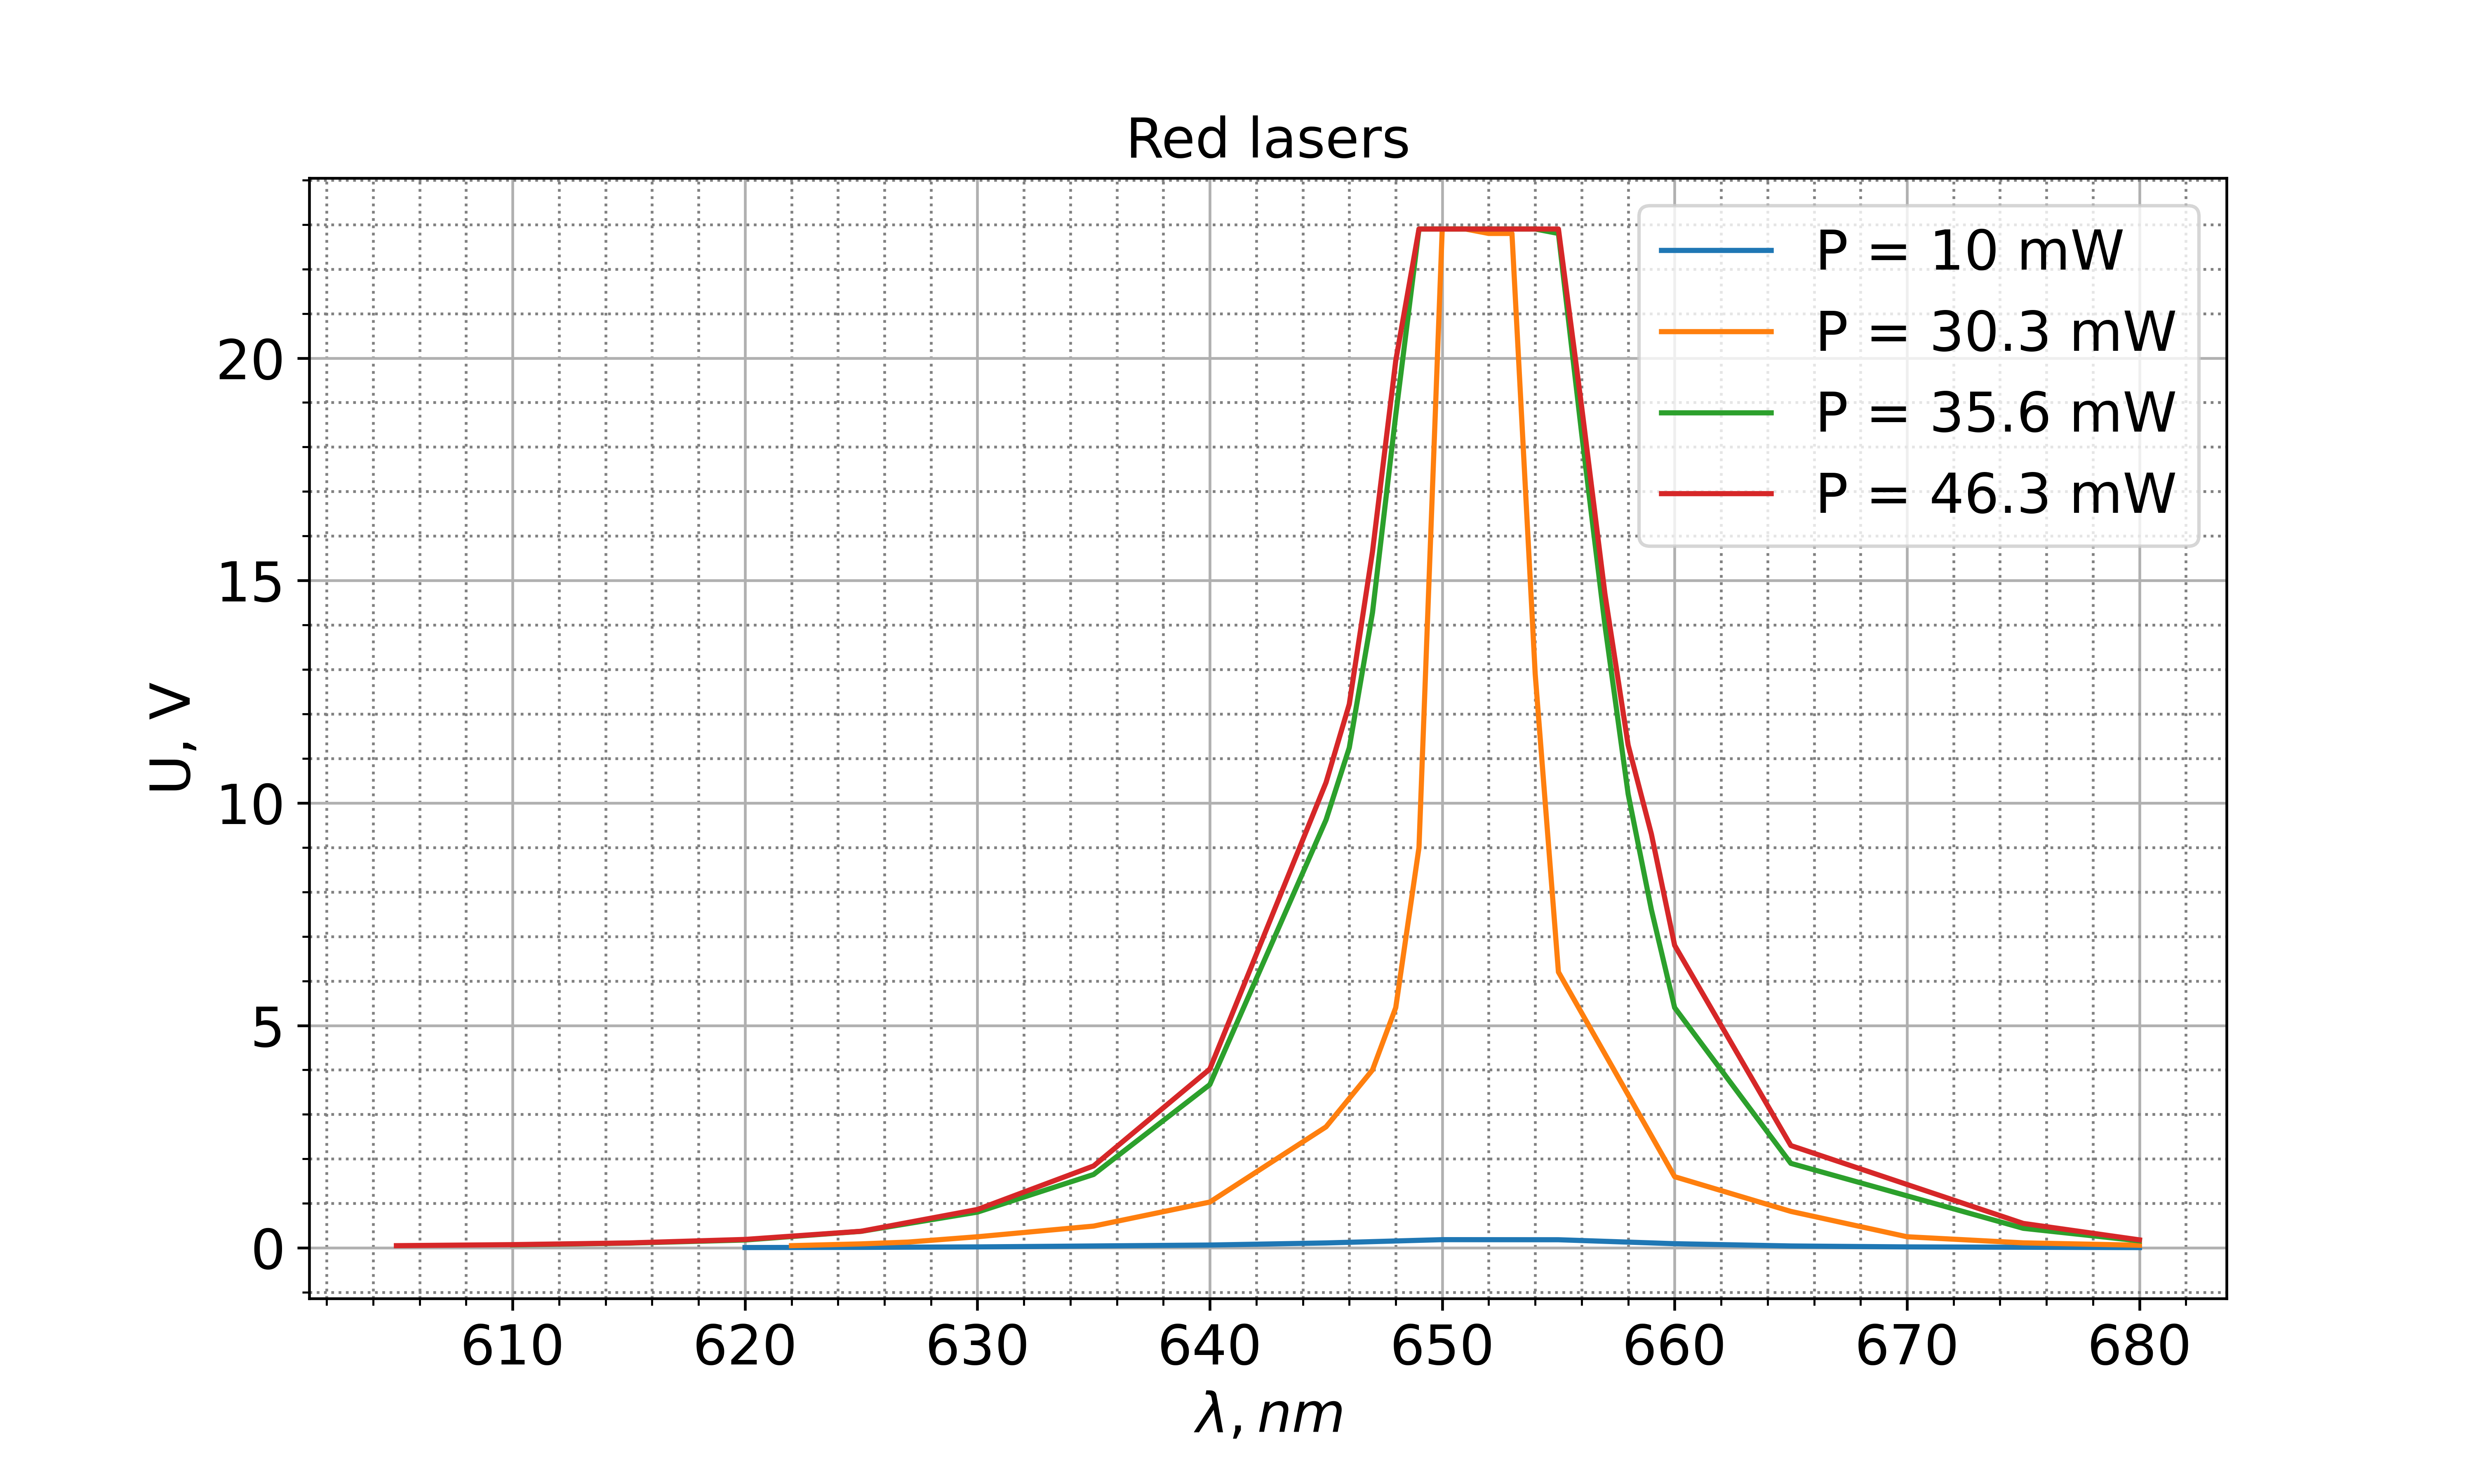
\includegraphics[scale=0.5]{spectr_red_lasers.png}
                \caption{Характеристика лазера при разных мощностях накачки}
                \label{lasers}
            \end{center}
        \end{figure}
        
        \par Заметно, что при уменьшении накачки аплитуда выходного излучения падает, что, вообще говоря, совершенно неудивительно. Длина волны генерируемого сигнала не зависит от {$I_{pump}$}.
        \par Незначительное повышение накачки может стать результатом значительного уширения полосы генерации.
        
        \par \textit{Аналогичные данные приведём для диодов}
        
        \begin{figure}[H]
            \begin{center}
                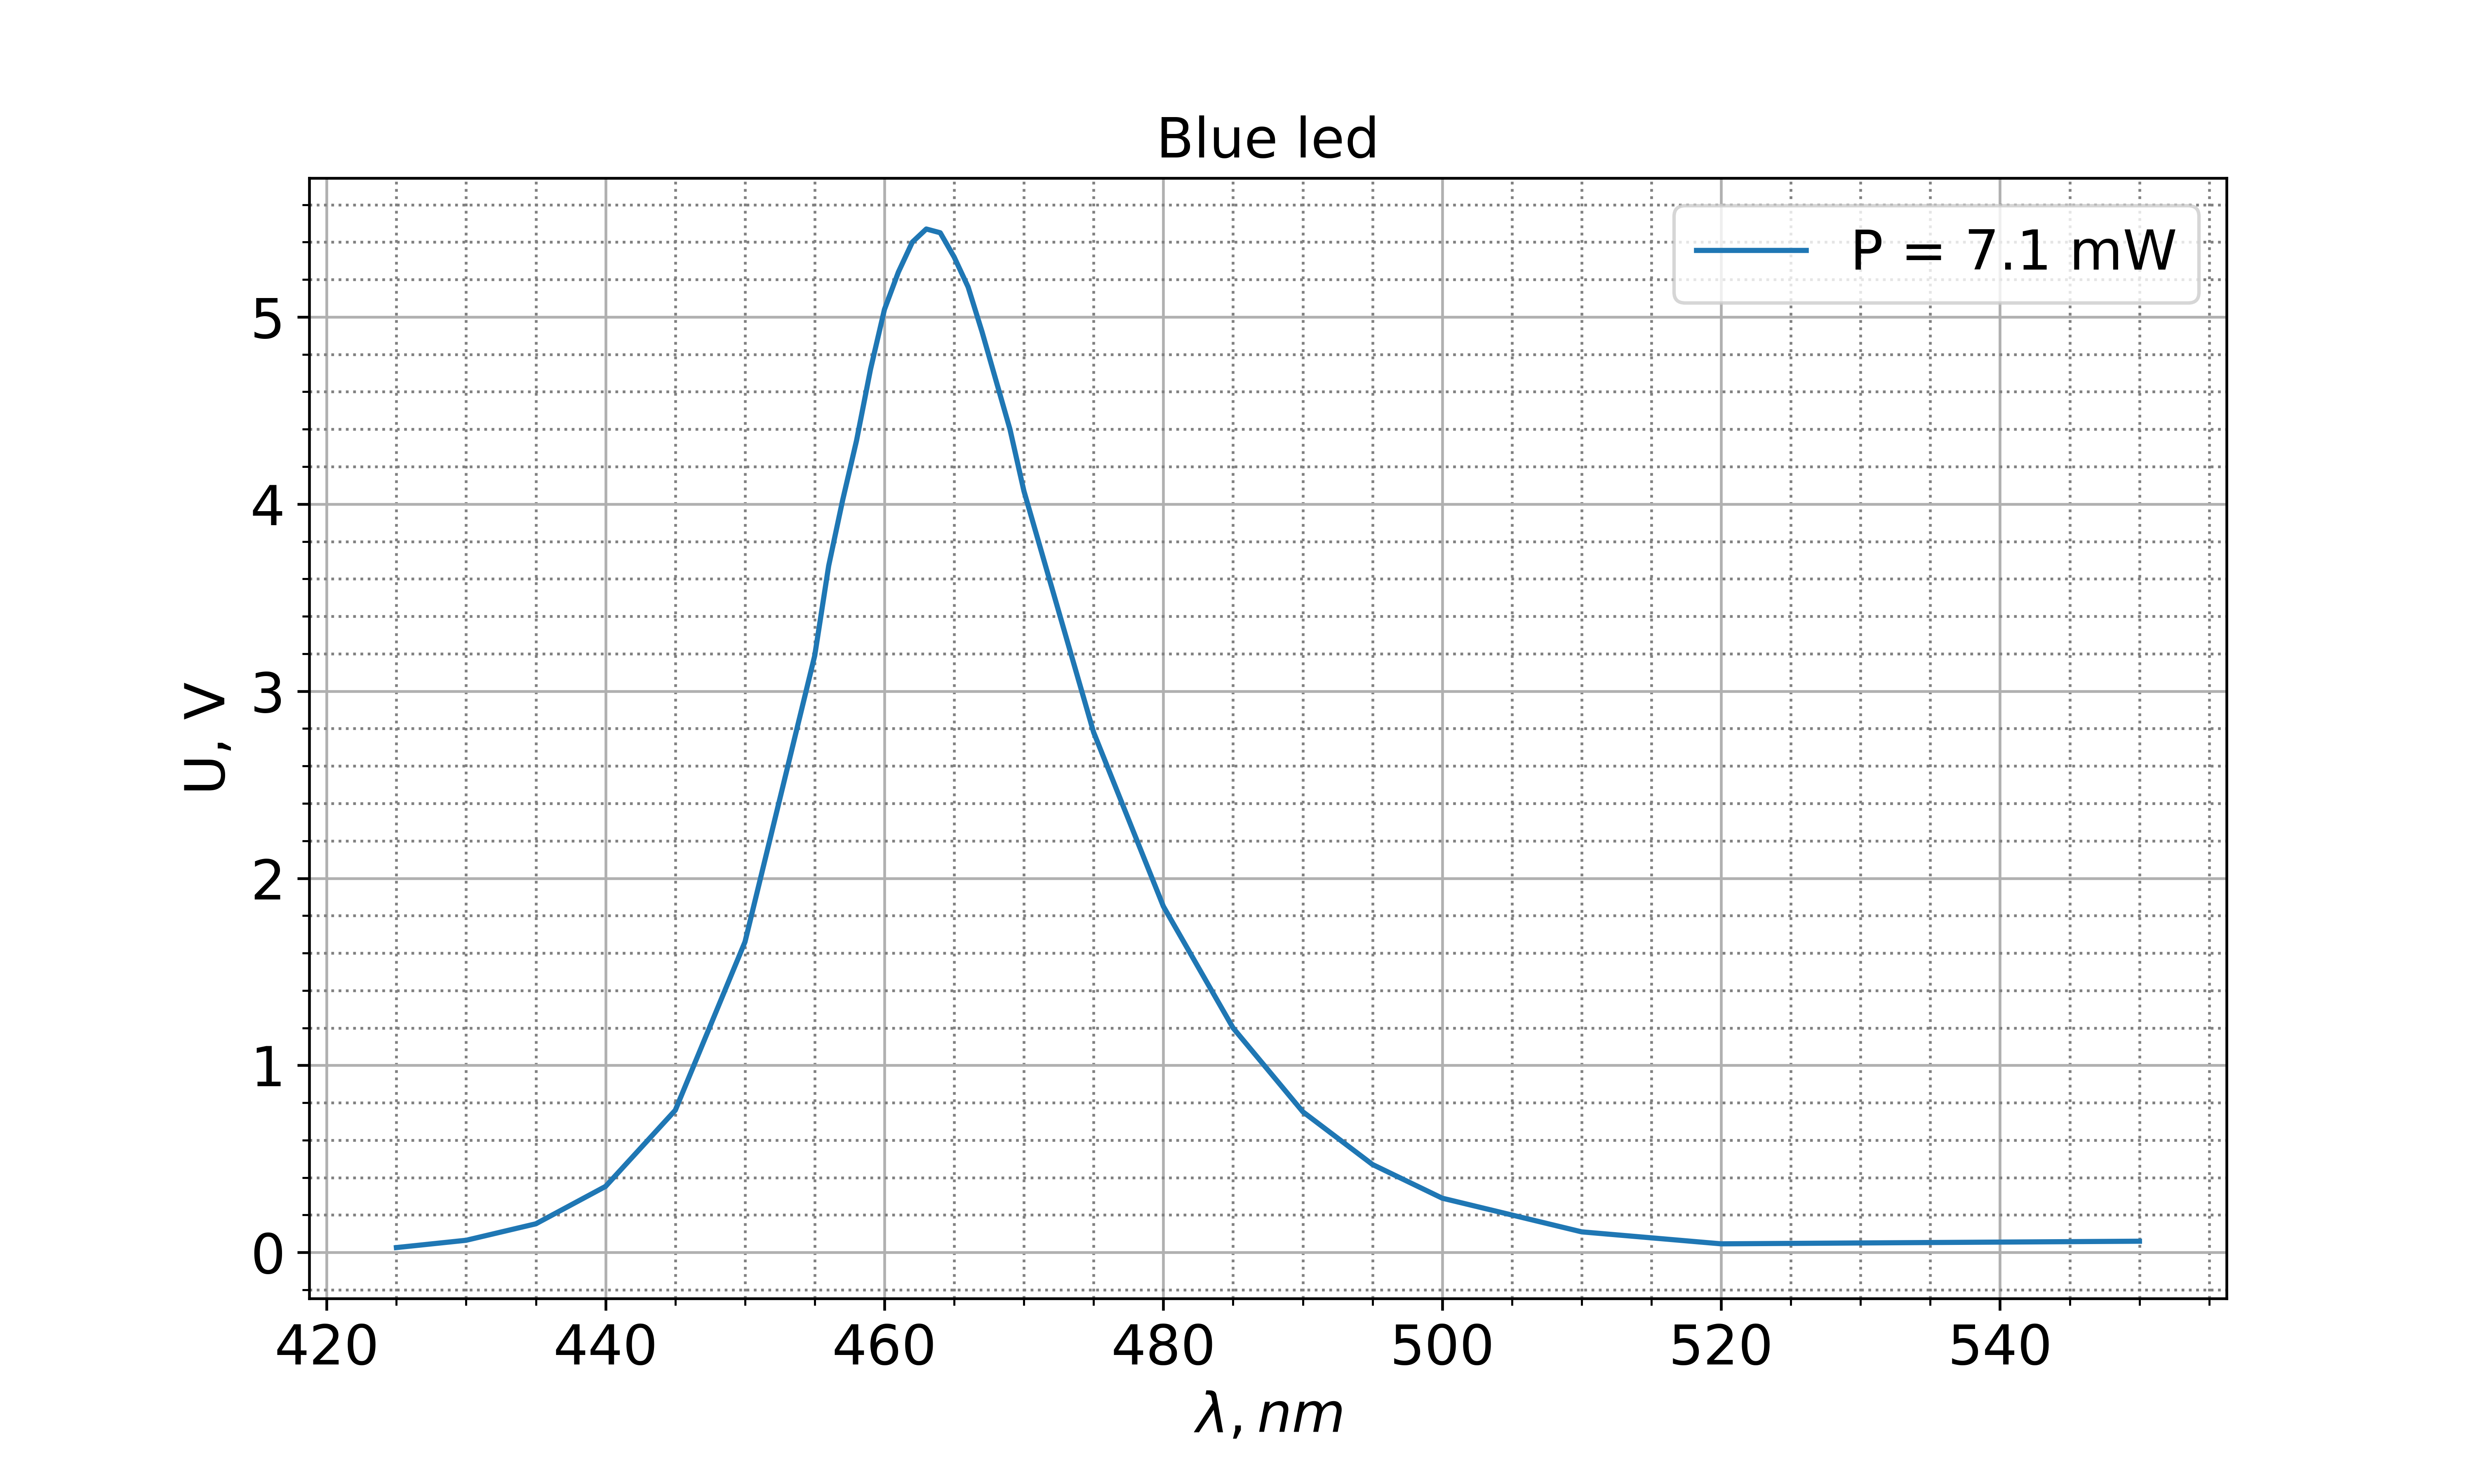
\includegraphics[scale=0.5]{spectr_blue_led.png}
                \caption{Характеристика синего диода}
                \label{blue}
            \end{center}
        \end{figure}

        \begin{figure}[H]
            \begin{center}
                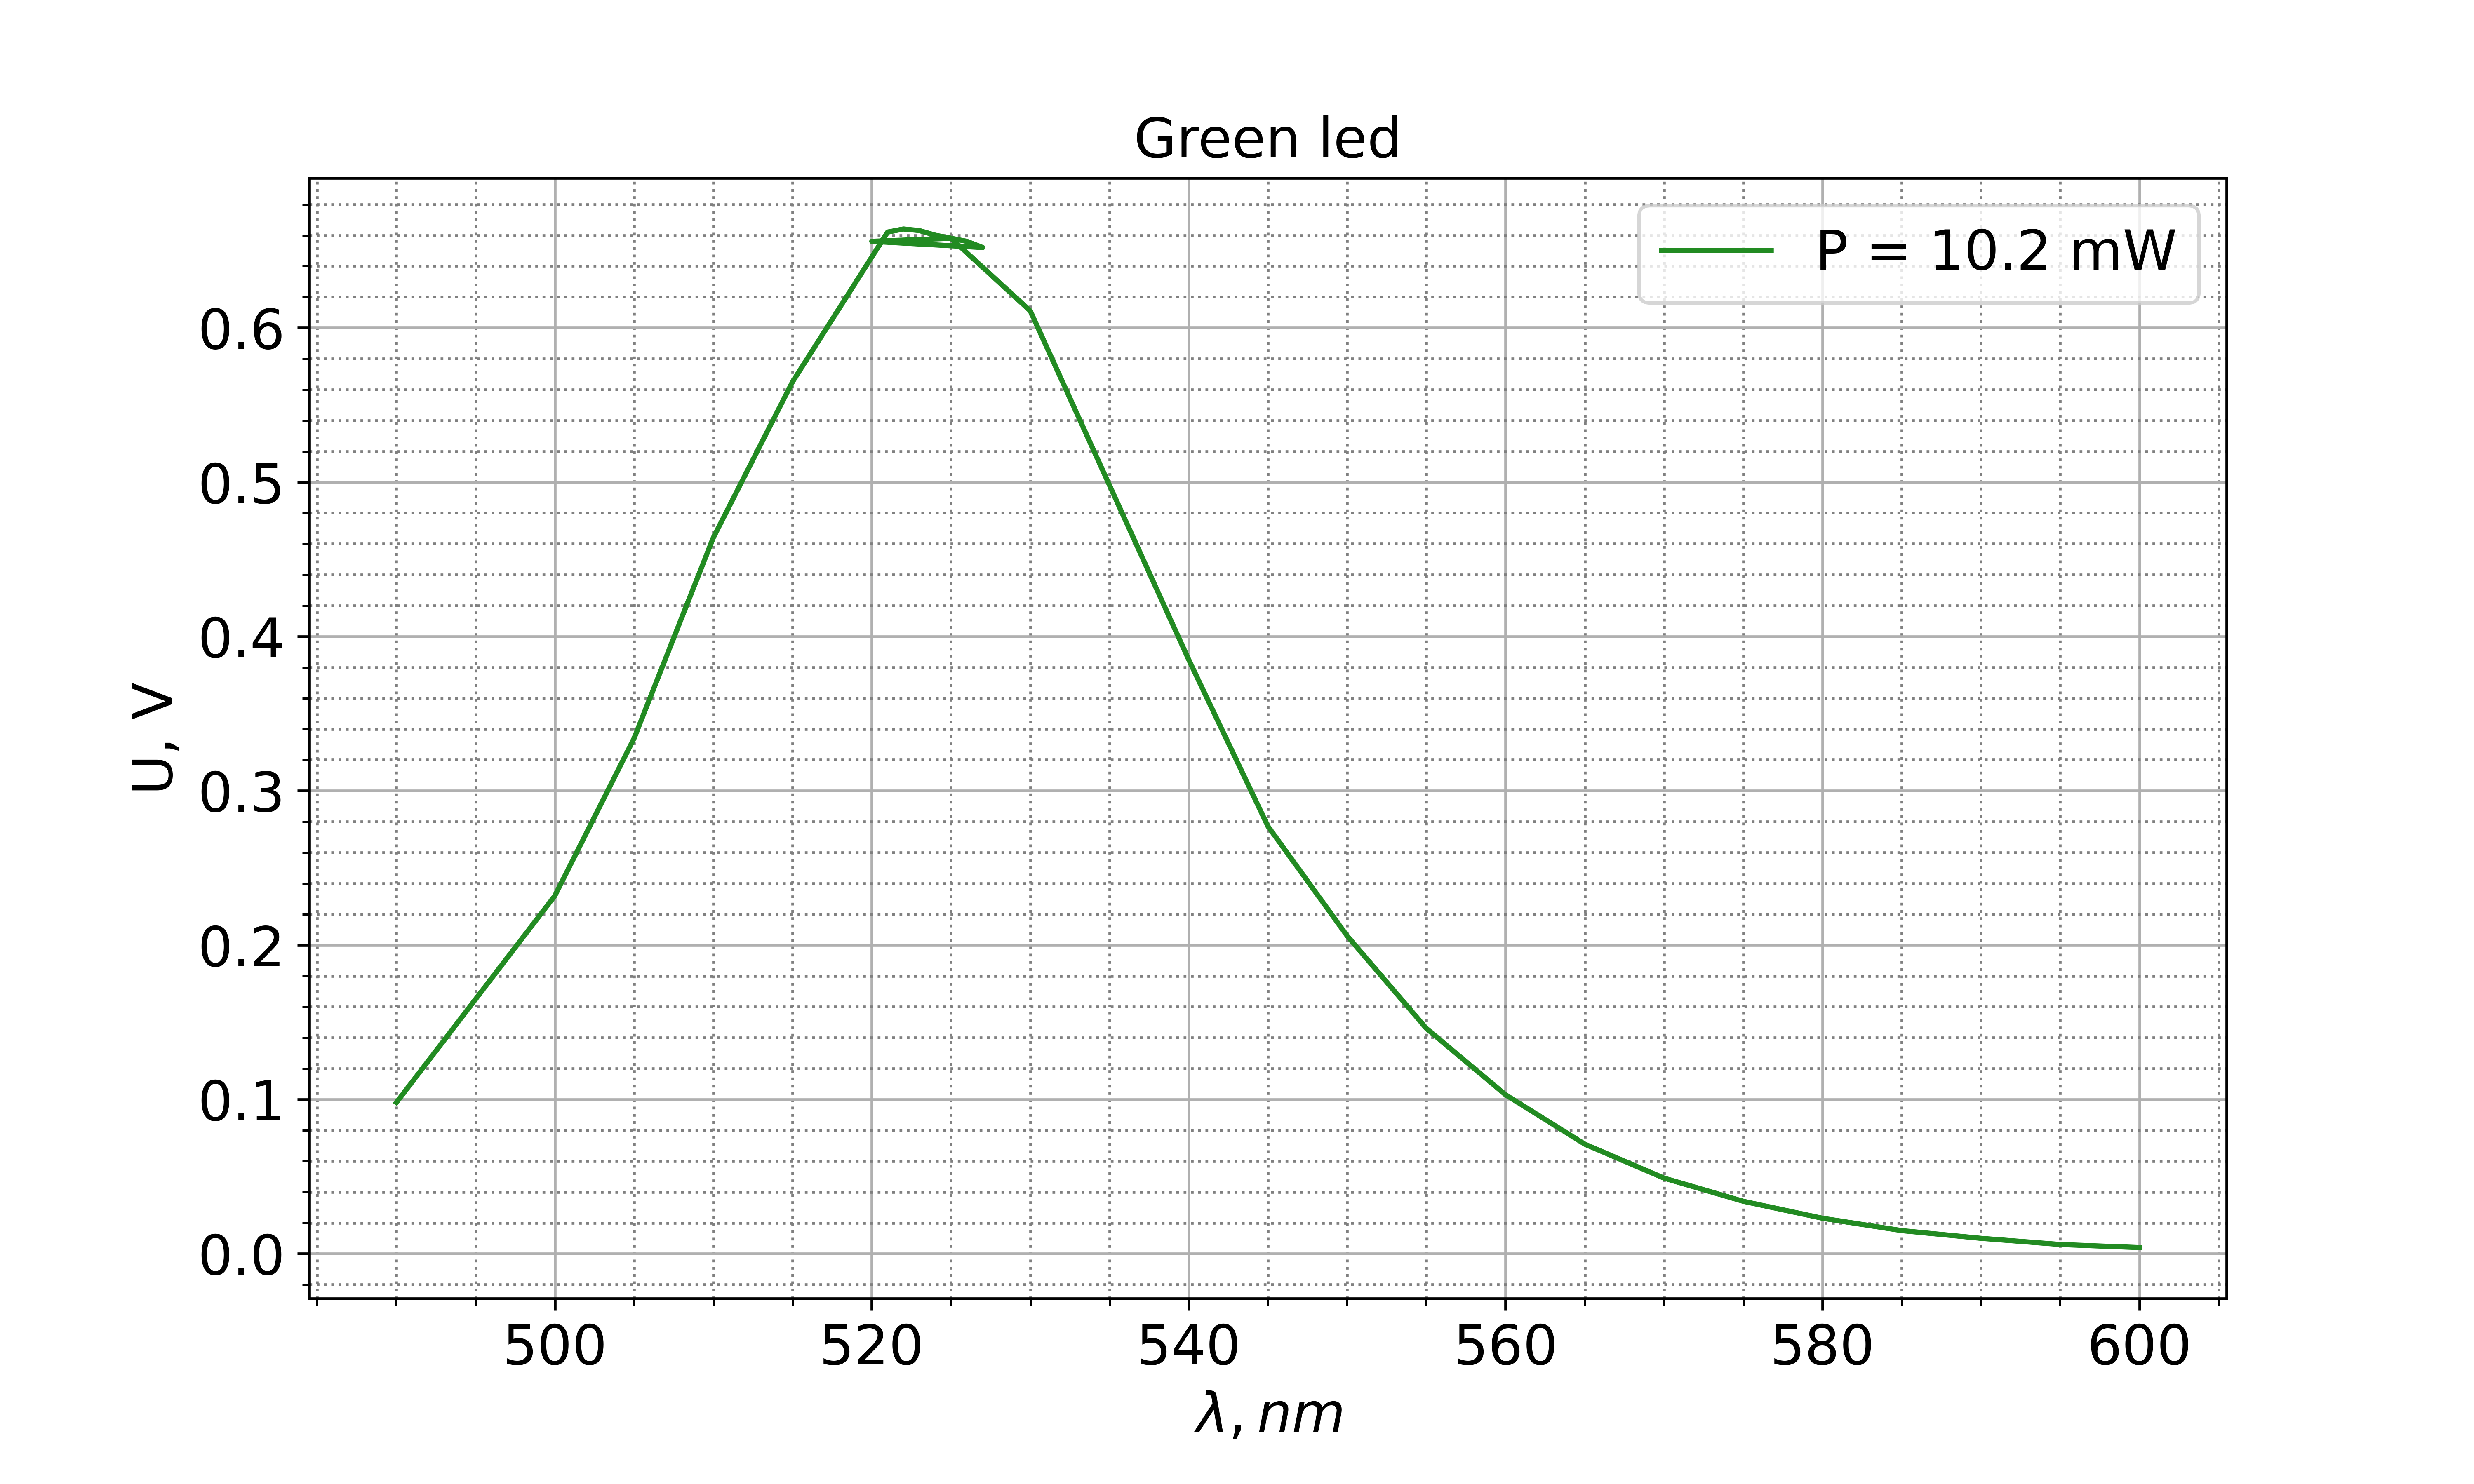
\includegraphics[scale=0.5]{spectr_green_led.png}
                \caption{Характеристика зеленого диода}
                \label{green}
            \end{center}
        \end{figure}

        \begin{figure}[H]
            \begin{center}
                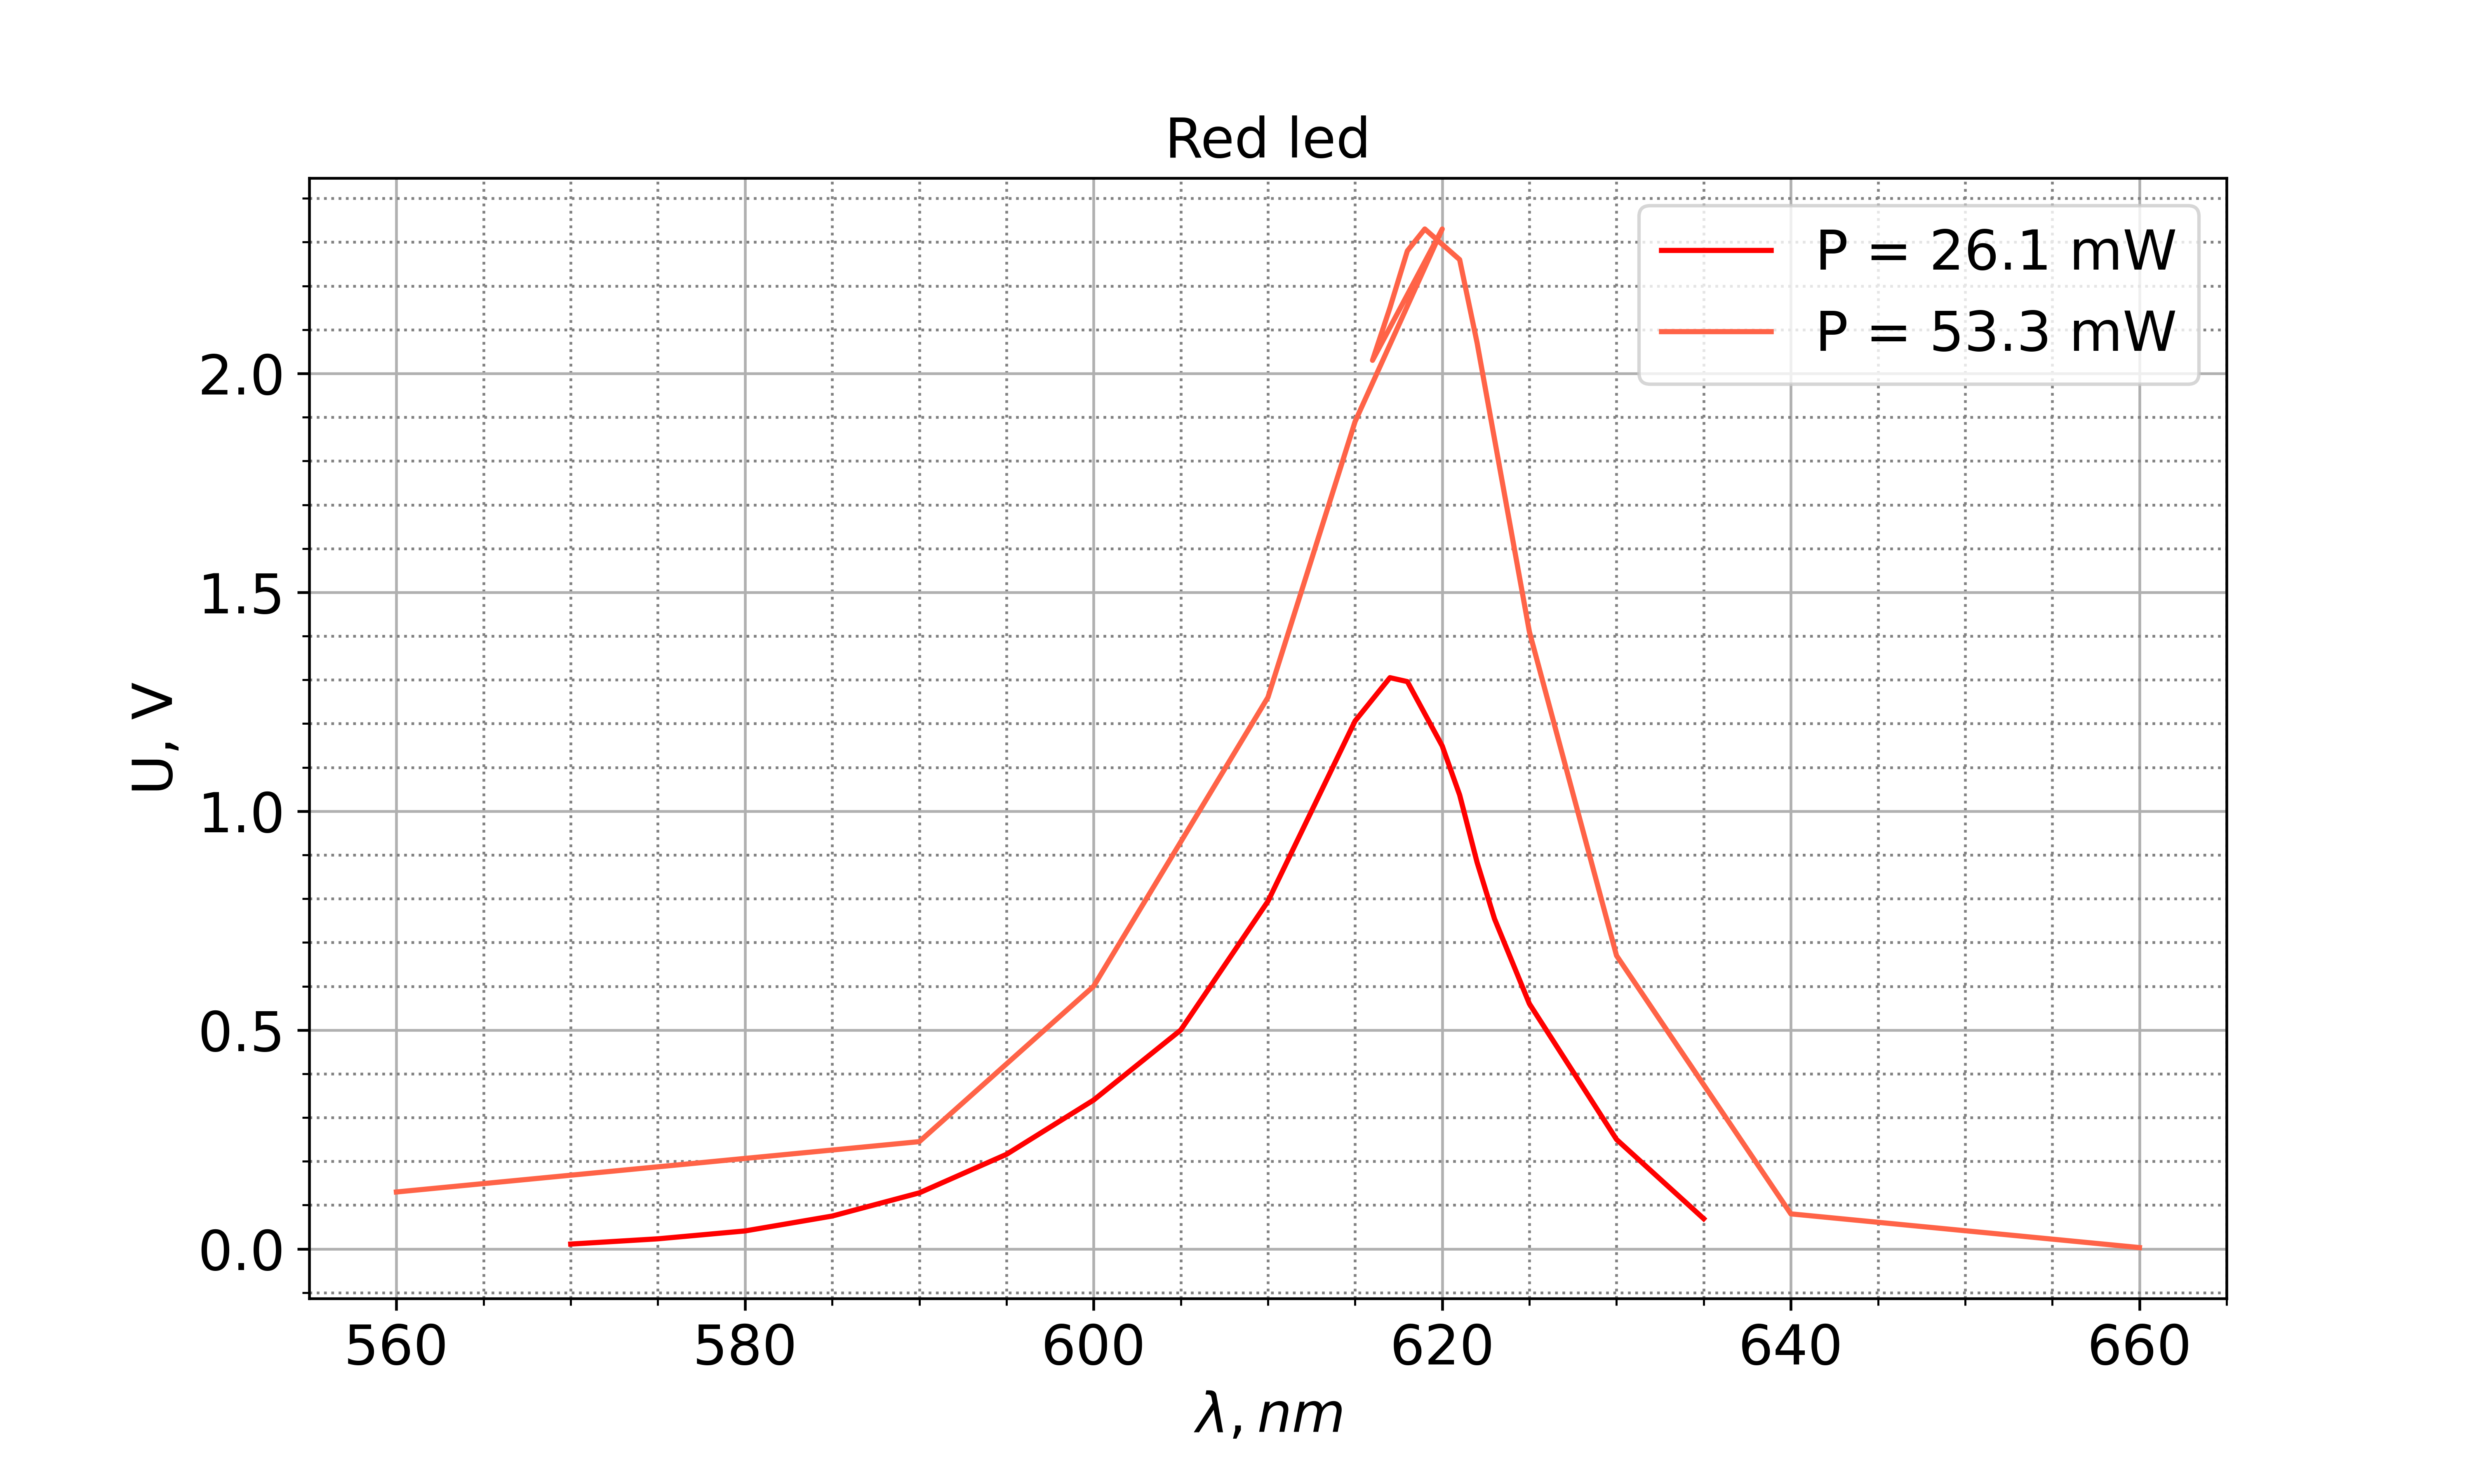
\includegraphics[scale=0.5]{spectr_red_led.png}
                \caption{Характеристика красного диода}
                \label{red}
            \end{center}
        \end{figure}
        
        \par Соответсвующи приблизительные максимумы излучения: \textcolor{red}{617}, \textcolor{green}{522}, \textcolor{blue}{462} nm.

	
	\subsection{Ватт-ваттные характеристики}
	
        \par \textit{Теперь рассмотрим зависимости амплитуды выходого сигнала от мощности накачки для двух лазеров}
        
        \begin{figure}[H]
            \begin{center}
                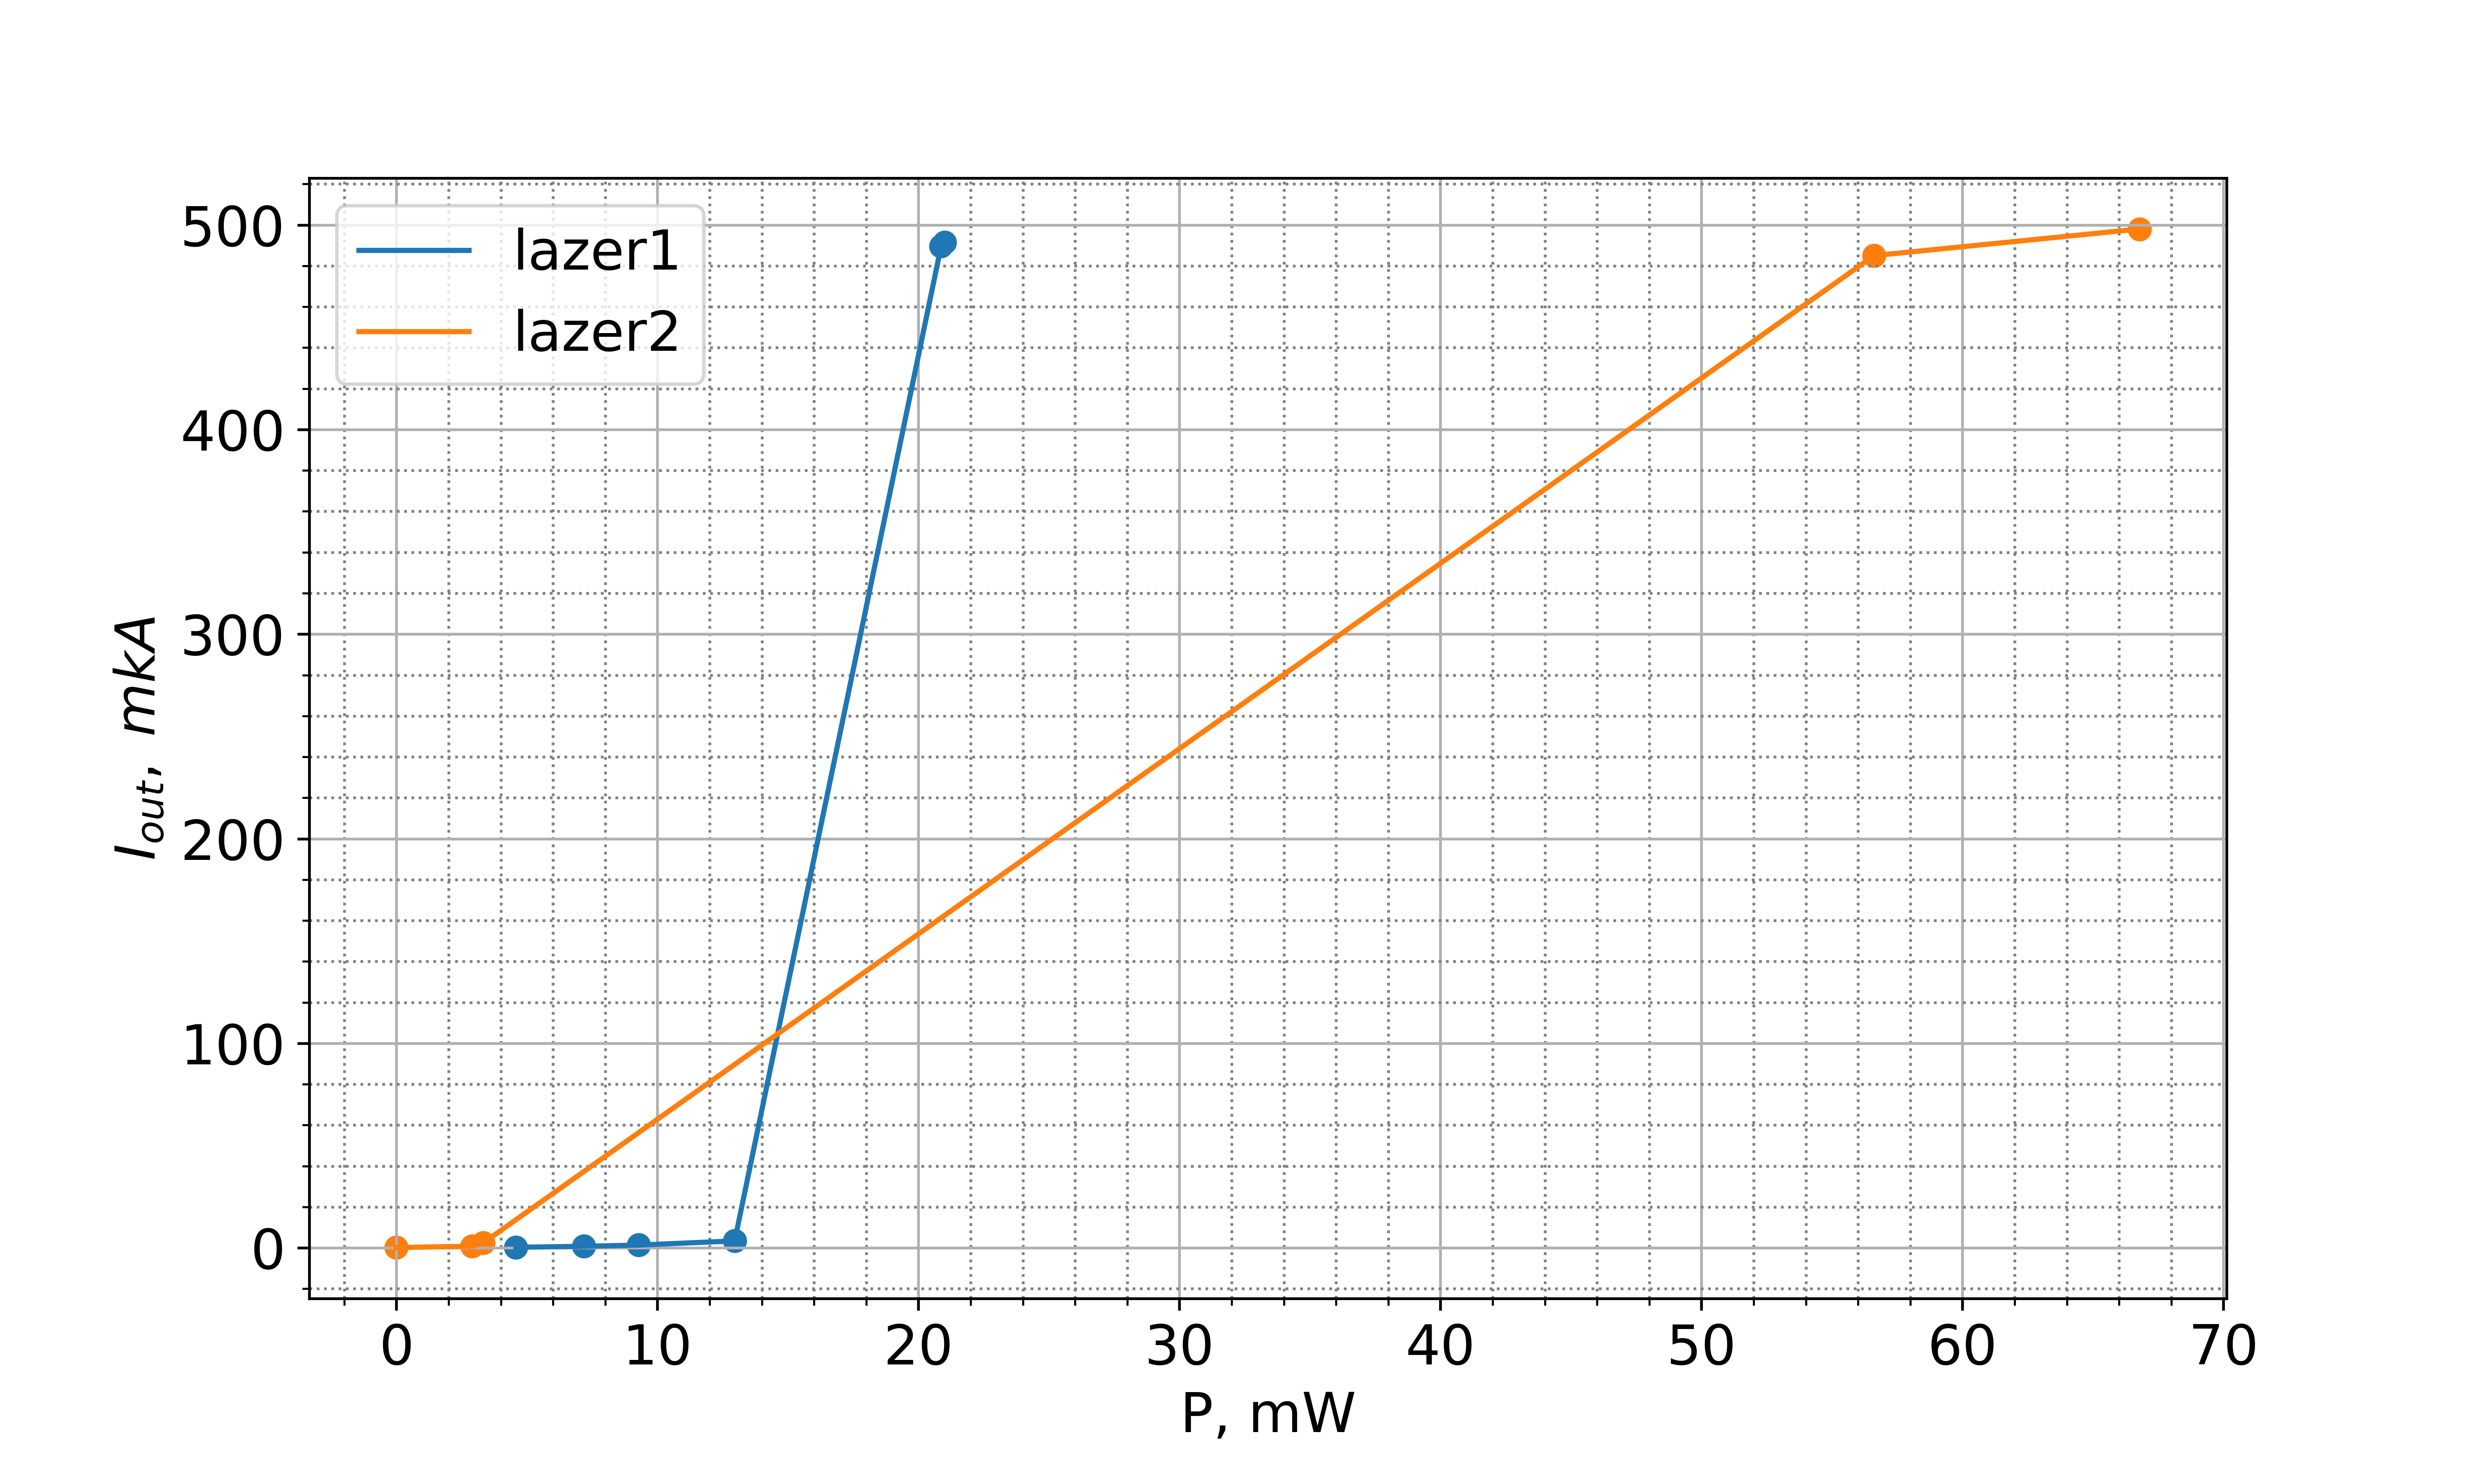
\includegraphics[scale=0.5]{WW-laser.png}
                \caption{В-В зарактеристика лазеров}
                \label{W-W-lasers}
            \end{center}
        \end{figure}
        
        \par На гарфике мы можем наблюдать три чётко выраженных участка: недостаток накачки (излучение остутсвует), линейная зависимость, насыщение (мощность излучения максимальна).\\
        Легко определить характерные значения, накачки, описывающие поеденя лазеров: пороговая мощность и мощность насыщения: {$P_{\mbox{порог}} \approx \textbf{23} \: \mbox{мВт}, \: P_{\mbox{нас}} \approx \textbf{45} \:  \mbox{мВт}$}. Про КПД лазера говорить не приходится, поскольку вместо мощности излуения детектировался лишь ток на фотодетекторе.
        
        \vspace{1cm}
        
        \par \textit{И для трёх диодов}
        
        \begin{figure}[H]
            \begin{center}
                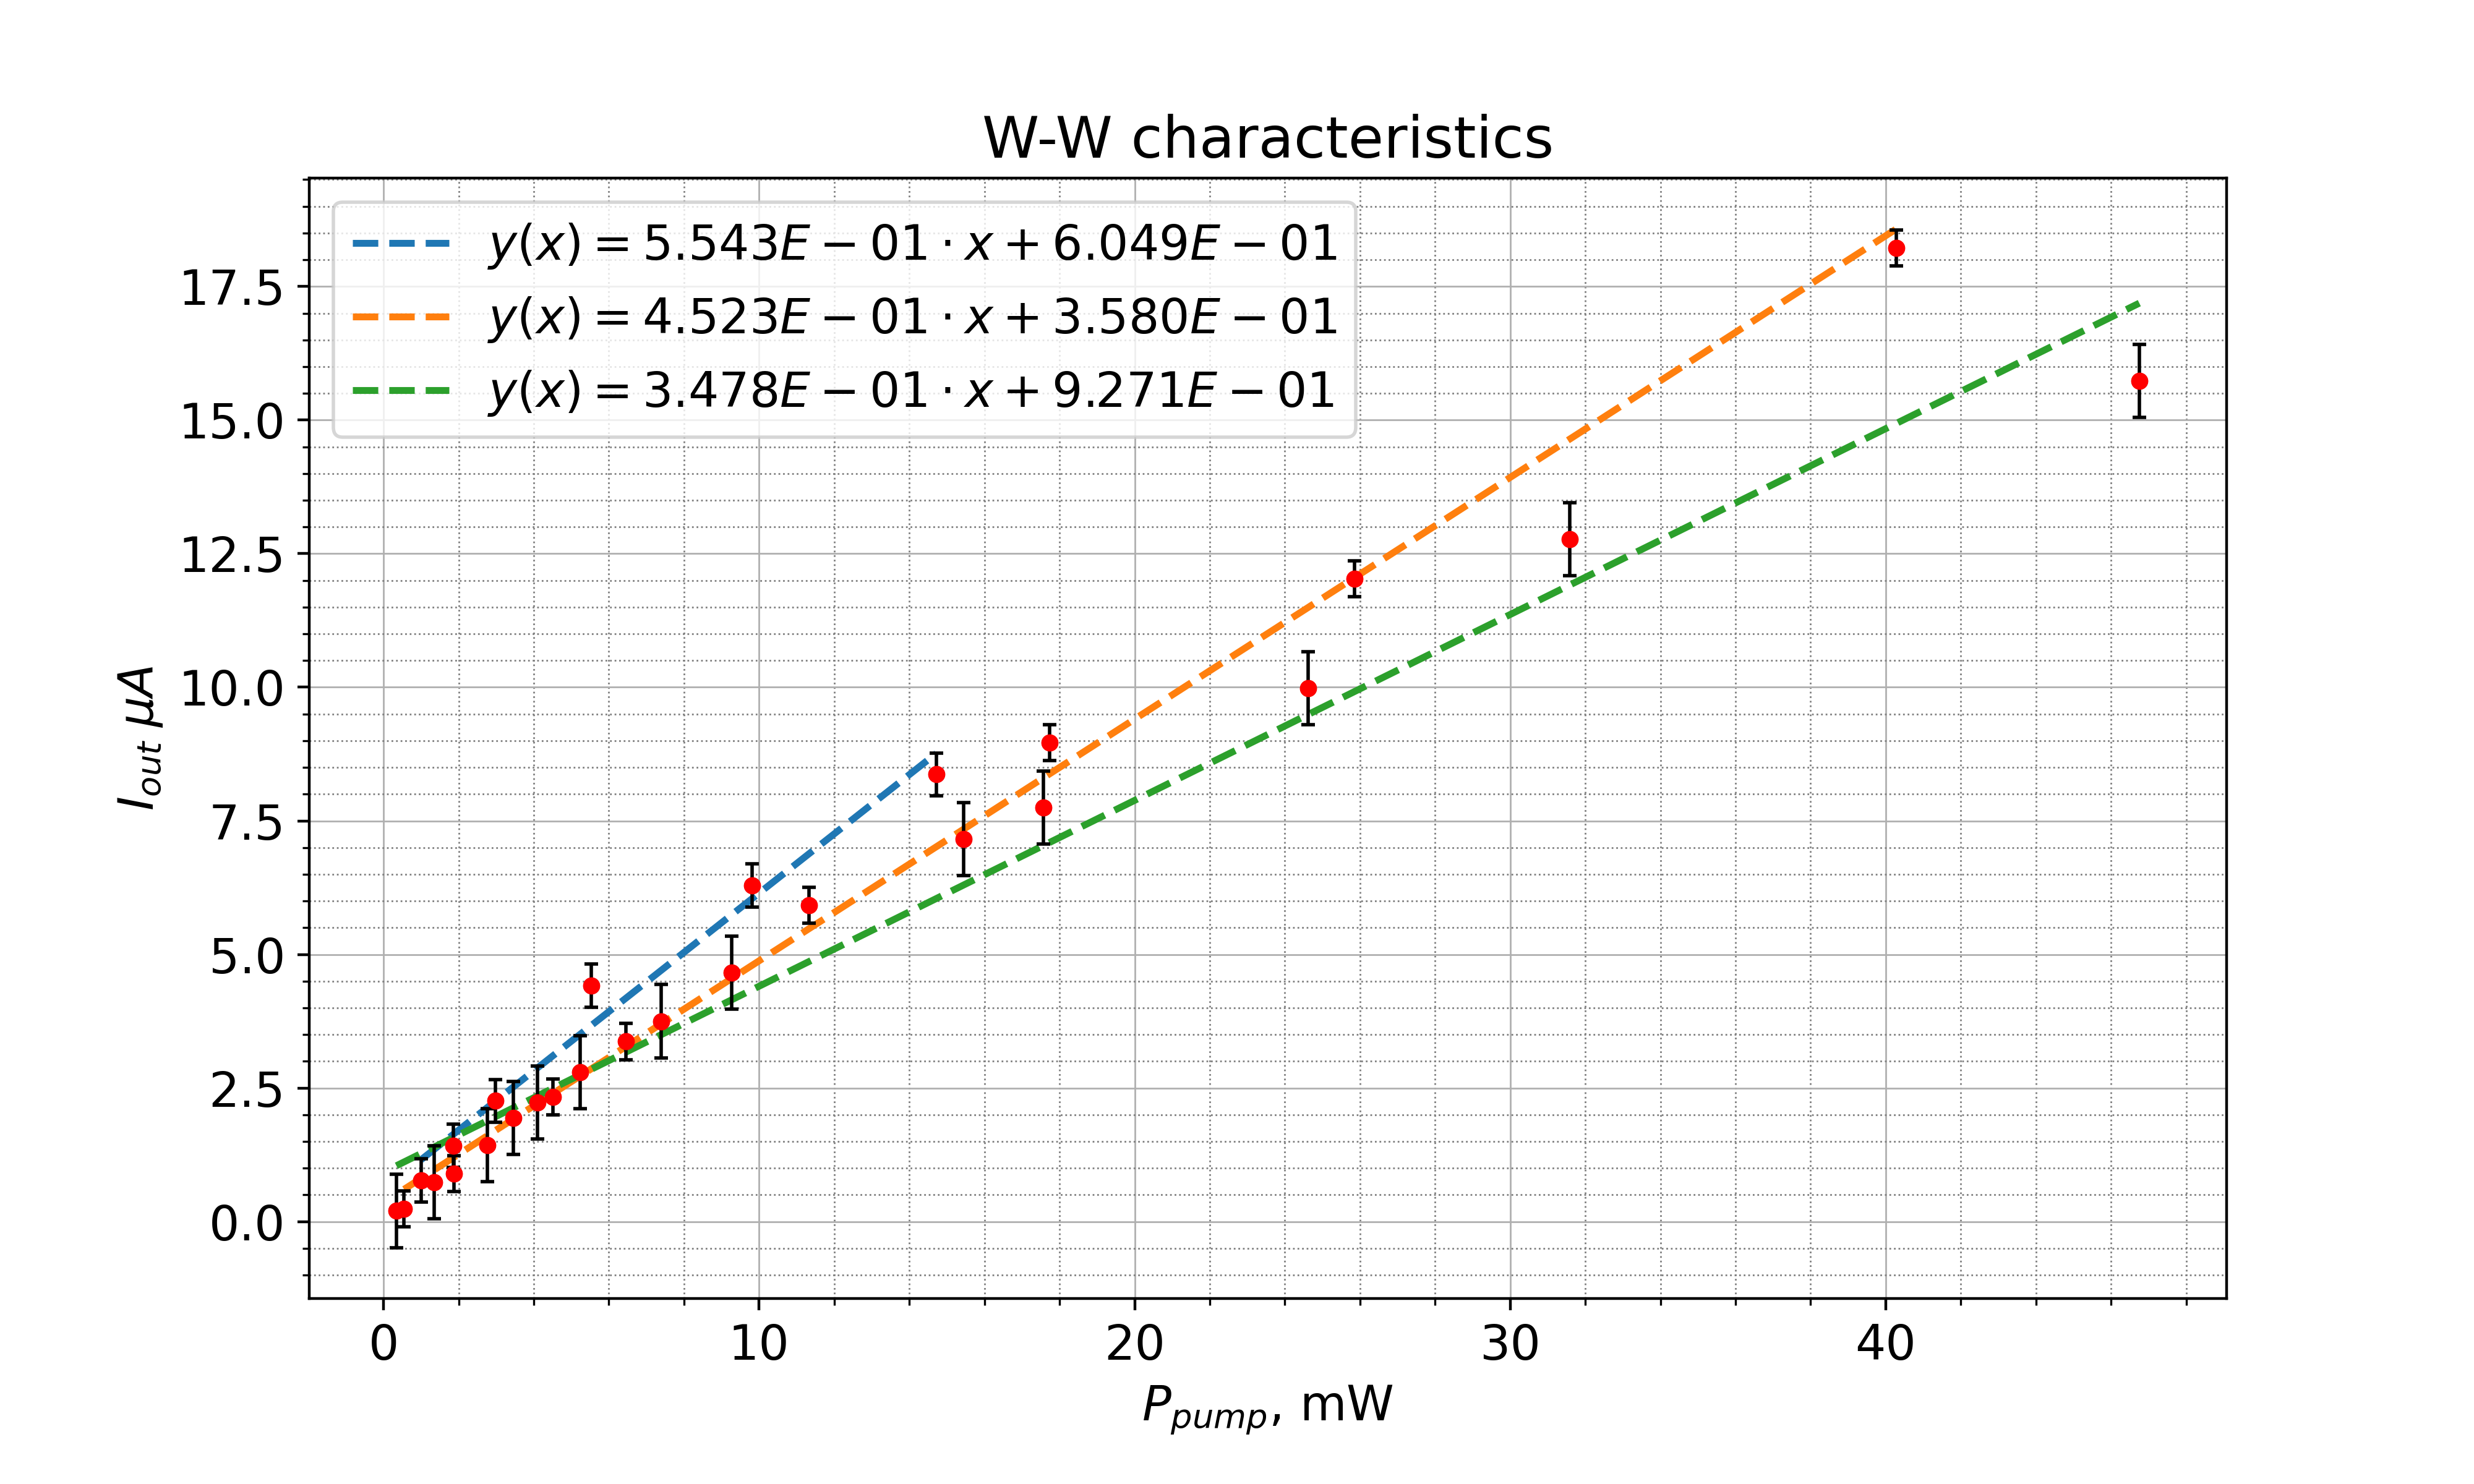
\includegraphics[scale=0.5]{W-W-led.png}
                \caption{Анимэ на картинке}
                \label{W-W-led}
            \end{center}
        \end{figure}
        
        \par В-В характеристика диодов имеет линейный вид, КПД каждого определяется как коэффициент наклона линейного фита, коэффициенты в таблицах (1,2,3)
        
        \begin{table}[H]
\centering
\caption{Коэффициенты аппроксимации Синего диода}
\label{coeffs_table}
\begin{tabular}{lrrr}
\toprule
coeffs &  coeffs\_values &  standard error &  relative se, \% \\
\midrule
   a\_0 &      5.543E-01 &       1.715E-03 &       3.094E-01 \\
   a\_1 &      6.049E-01 &       1.020E-01 &       1.686E+01 \\
\bottomrule
\end{tabular}
\end{table}

        \begin{table}[H]
\centering
\caption{Коэффициенты аппроксимации красного богатыря}
\label{coeffs_table}
\begin{tabular}{lrrr}
\toprule
coeffs &  coeffs\_values &  standard error &  relative se, \% \\
\midrule
   a\_0 &      4.523E-01 &       1.139E-04 &       2.518E-02 \\
   a\_1 &      3.580E-01 &       3.985E-02 &       1.113E+01 \\
\bottomrule
\end{tabular}
\end{table}

        \begin{table}[H]
\centering
\caption{Коэффициенты аппроксимации зеленого диода}
\label{coeffs_table}
\begin{tabular}{lrrr}
\toprule
coeffs &  coeffs\_values &  standard error &  relative se, \% \\
\midrule
   a\_0 &      3.478E-01 &       2.382E-04 &       6.849E-02 \\
   a\_1 &      9.271E-01 &       8.325E-02 &       8.979E+00 \\
\bottomrule
\end{tabular}
\end{table}

        
        \newpage
    
\section{Выводы}

    \par Полученные результаты позволяют сформулировать следующие тезисы:

        \begin{enumerate}
            \item Рост мощность накачки увеличивает ширину спектра излучения лазера, не меняя частоту генерации;
            \item Рост мощность накачки увеличивает ширину спектра излучения диода, снижая частоту генерации;
            \item Лазер имеет наименьшую ширину спектра излучения при сравнимых мощностях накачки;
            \item Диоды имеют линейную ватт-ваттную характеристику по крайней мере в диапазоне от 0 до {$\approx50$} мВт;
            \item Лазер имеет линейную ВВХ искючительно в заданном диапазоне мощностей накачки, от 23 до 45 мВт. Границы диапазона называются {$\textit{пороговой мощностью}$} и {$\textit{мощностью насыщения}$} соответсвенно;
            \item Коэффициенты полезного действия для изучаемых диодов: \textcolor{red}{45\%}, \textcolor{green}{35\%}, \textcolor{blue}{55\%}.
        \end{enumerate}
    



\end{document}